\begin{minipage}{0.50\textwidth}
    \begin{lstlisting}[style=CStyle]
#include <cstdint>

uint32_t 
computeLoan(bool isHouseLoan, 
                int principal) {
  //EBB
  uint32_t
  baseRate = principal * 2 / 100;

  if (isHouseLoan) {
    // TBB
    baseRate = principal * 5 / 100;
  } else {
    // FBB
    baseRate = principal * 7 / 100;
  }

  // TailBB
  return (baseRate + 5) / 10 * 10;
}
    \end{lstlisting}
\end{minipage}%
\hspace{1cm} % Adjust horizontal overlap
\begin{minipage}{0.40\textwidth}
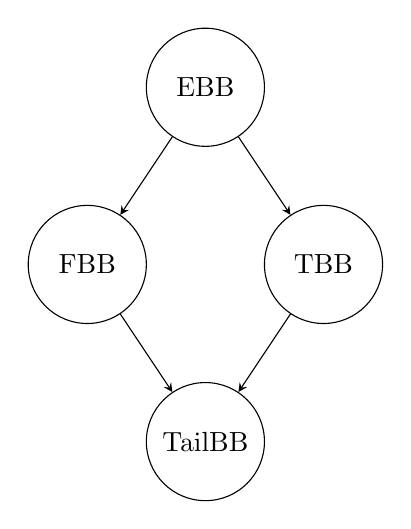
\begin{tikzpicture}[node distance=2cm and 3cm, >=stealth]
    % Style for consistent node dimensions
    \tikzstyle{node} = [circle, draw, fill=white, minimum size=1.5cm, inner sep=0]

    % Nodes
    \node[node] (EBB) at (1.5, 4.5) {EBB};
    \node[node] (TBB) at (3, 2.25) {TBB};
    \node[node] (FBB) at (0, 2.25) {FBB};
    \node[node] (TailBB) at (1.5, 0) {TailBB};

    % Edges
    \draw[->] (EBB) -- (TBB);
    \draw[->] (EBB) -- (FBB);
    \draw[->] (TBB) -- (TailBB);
    \draw[->] (FBB) -- (TailBB);
\end{tikzpicture}
\end{minipage}